\documentclass[10pt]{beamer}

\usetheme{metropolis}
\usepackage{appendixnumberbeamer}


\usepackage{ulem}

\usepackage{booktabs}
\usepackage[scale=2]{ccicons}

\usepackage{pgfplots}
\usepgfplotslibrary{dateplot}

\usepackage{xspace}
%\usepackage{listings}
\input{listing_js.tex}
\newcommand{\themename}{\textbf{\textsc{metropolis}}\xspace}

\setbeamercolor{alerted tex}{fg=red,bg=blue}
\setbeamercolor{progress bar}{fg=red, bg=blue}
    %use=alerted text,
    %fg=alerted text.fg,
    %bg=alerted text.fg!50!black!30
%}

\title{Remote20/20}
\subtitle{Remote (but connected) psychophysics}
\date{\today}
\author{Daniel R. Coates}
\institute{University of Houston College of Optometry}
\titlegraphic{\hfill\includegraphics[height=1.5cm]{uhlogo.png}}

\usepackage{pdfpc-commands}

\begin{document}

\maketitle

\begin{frame}{Table of contents}
  \setbeamertemplate{section in toc}[sections numbered]
  \tableofcontents[hideallsubsections]
\end{frame}

\begin{frame}{Fundamentally peer-to-peer}
    \begin{tabular}{l|l}
        Them & Us \\
        \hline
	{\hfill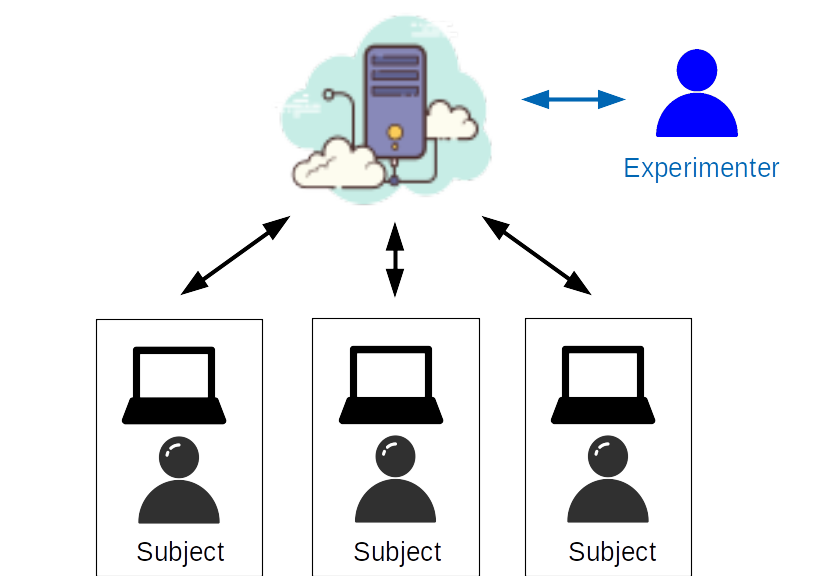
\includegraphics[width=5cm]{../doc/clouds_openloop.png}}   &
        \pause
	{\hfill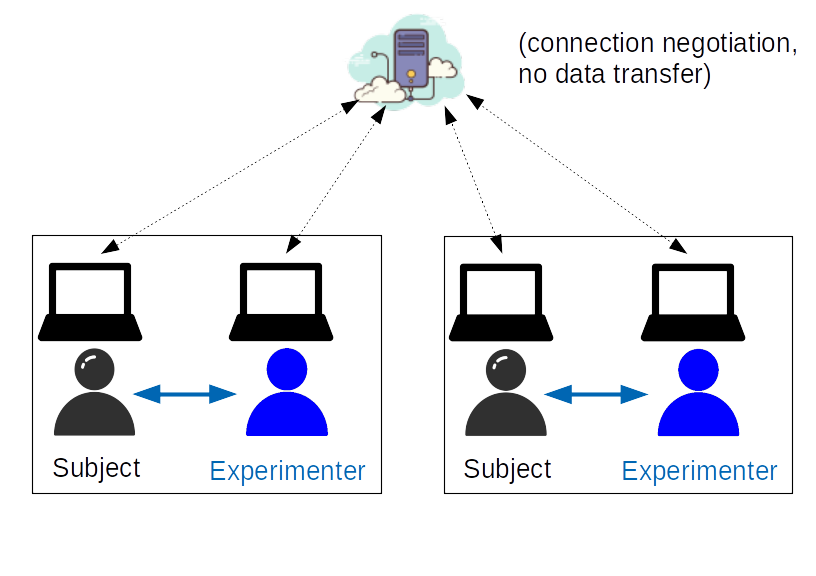
\includegraphics[width=5cm]{../doc/pairs.png}}   \\
	\end{tabular}
\end{frame}

\section{Use cases}

\begin{frame}{Optometry teaching labs}
	\begin{itemize}[<+->]
        \item Optometry teaching labs (UHCO and UC Berkeley)
        \item Experiental introduction to:
	        \begin{itemize}
                \item Psychophysical procedures
                \item \textit{Low-level} visual perception
                \begin{itemize}
                    \item Contrast sensitivity function, dark adaptation, increment thresholds, summation
            \end{itemize}
            \end{itemize}
        \item Our lab systems (HW\&SW) were due for overhaul anyway, as well as having new COVID-19 constraints
    \end{itemize}
\end{frame}

\begin{frame}{``Connected'' remote experiments}
	\begin{itemize}[<+->]
        \item For our research (visual crowding, stereo vision, eye movements), experimenter is pretty ``hands-on'' with subjects
        \item Use few subjects (often colleagues or classmates), running more trials and longer blocks
        \item This ``style'' is essential to test certain populations (e.g. low vision)
        \item COVID-19 \& social distancing prevented close contact
    \end{itemize}
\end{frame}

\begin{frame}{Fundamentally peer-to-peer}
    \begin{tabular}{l|l}
        Them & Us \\
        \hline
	{\hfill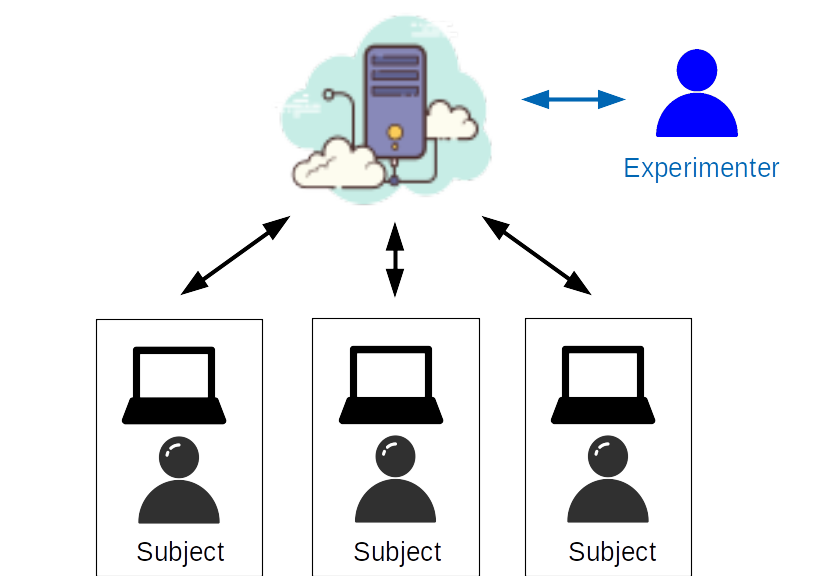
\includegraphics[width=5cm]{../doc/clouds_openloop.png}}   &
	{\hfill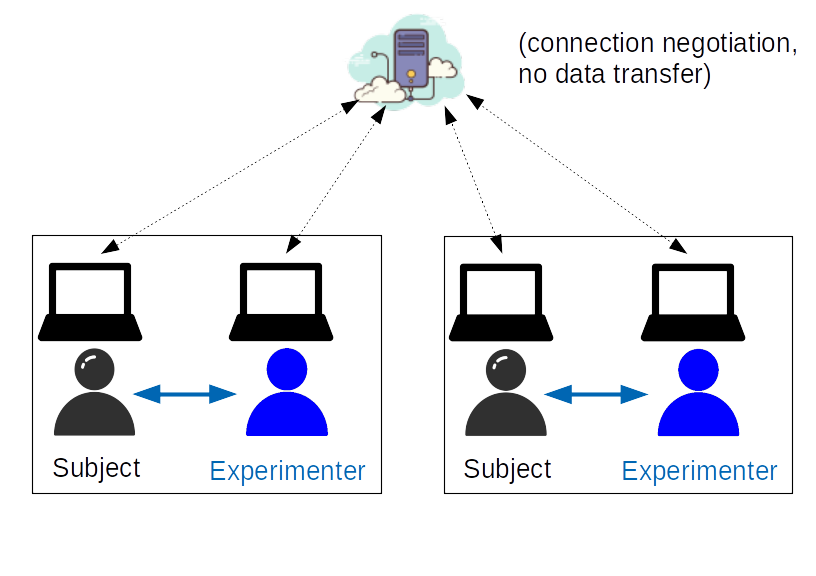
\includegraphics[width=5cm]{../doc/pairs.png}}   \\
	\end{tabular}
\end{frame}


\section{What does it look like?}
\begin{frame}{Dark adaptation lab}
    \begin{center}
    \inlineMovie[loop]{da_cropped_mute.mp4}{da1.png}{height=0.8\textheight}
    \end{center}
\end{frame}
\begin{frame}{Psychophysical methods lab}
    \begin{center}
    \inlineMovie[loop]{vs205.mp4}{vs205.png}{height=0.8\textheight}
    \end{center}
\end{frame}
\begin{frame}{Crowding Experiment (NIH/NEI T35 Summer 2020 Project)}
    \begin{center}
    \inlineMovie[loop]{crowdcrop.mp4}{crowdcrop.png}{height=0.82\textheight}
    \end{center}
\end{frame}

\iffalse
\begin{frame}{Results: In-lab crowding study}
    \begin{columns}[c]
        \column{.25\textwidth}
    \includegraphics[height=2.5cm]{t35_setup2.png}
        \column{.7\textwidth}
    \includegraphics[height=4cm]{all_mocs_raw.png}
  \end{columns}
\end{frame}
\fi

\begin{frame}{Results: In-lab crowding study}
    \begin{center}
    \includegraphics[height=3.25cm]{t35_setup2.png}
        \pause
    \includegraphics[height=4.8cm]{all_mocs_raw.png}
    \end{center}
\end{frame}


\begin{frame}{Results: Labs}
    \begin{columns}[c]
        \column{.4\textwidth}
    \includegraphics[height=7cm]{a25.png}
        \column{.5\textwidth}
        \includegraphics[height=7cm]{mocs.png}
  \end{columns}
\end{frame}

\section{How it works}

\begin{frame}{How it works}
    \begin{itemize}[<+->]
        \item \textbf{Javascript, HTML/CSS}
        \item \textbf{PeerJS} for peer-to-peer connectivity
            \begin{itemize}[]
                \item Open-source library built on top of WebRTC
                \item Abstraction layer makes p2p connections simple
            \end{itemize}
        \item \textbf{Javascript Animation, HTML5 Canvas, WebGL} for drawing
            \begin{itemize}
                \item Javascript animation allows per-frame update (60Hz)
                \item WebGL shaders allows fast, precise control of each pixel (e.g. bit stealing)
            \end{itemize}
    \end{itemize}
\end{frame}

% Using typewriter font: \ttfamily inside \lstset
\begin{frame}[fragile]{Execution modes}
    %\lstset{language=Javascript}
                %basicstyle=\ttfamily,
                %keywordstyle=\color{blue}\ttfamily,
                %stringstyle=\color{red}\ttfamily,
                %commentstyle=\color{green}\ttfamily,
                %morecomment=[l][\color{magenta}]{\#}
%}

Parameter strings for specialty ``run-forever'' widgets
\begin{lstlisting}[language=JavaScript]
"G 0.25 0.8 0 0 0.1" // Show single low-frequency grating of given size, contrast, color, flash rate, etc.
\end{lstlisting}

Javascript code sent to device for remote execution (can be
    edited/debugged/run) \textit{in the browser}!  

\begin{lstlisting}[language=JavaScript]
clear('#ffffff');
fixation(0,-700,40,4,'green',style='+');
flip(30);

clear('#ffffff');
//beep(1,880,30);
fixation(0,-700,40,4,'black',style='+');
draw_letter('E',${orientation},0,333,${size},'black',-1,-1);
flip(10);	//Draw for 10 frames (166ms);

clear('#ffffff');
fixation(0,-700,40,4,'black',style='+');flip(1);
\end{lstlisting}
    Can be edited/debugged/run in the browser!
\end{frame}


\begin{frame}{Javascript animation loop performance}
\end{frame}

%\begin{frame}{Two execution modes: monolithic and scripted}
    %\begin{itemize}[<+->]
        %\item \textbf{Javascript}, HTML/CSS

\section{Demo}

\section{Current status \& limitations}
\begin{frame}{Current status \& limitations}
    \begin{itemize}[<+->]
		\item API changing rapidly!
		\item Browser/platform issues
	        \begin{itemize}
                \item \textcolor{red}{\sout{iPad/iPhone}}
            \end{itemize}
        \item Networking issues (firewalls, etc.)
        \item Security
    \end{itemize}
\end{frame}

\begin{frame}[standout]
  Thank you! \\
    Questions? \\ \vspace{0.5in}
    \url{http://github.com/dcoates/remote2020} \\
  drcoates@uh.edu \\
  remote2020@coateslab.org
\end{frame}

\end{document}
